%package list
\documentclass{article}
\usepackage[top=3cm, bottom=3cm, outer=3cm, inner=3cm]{geometry}
\usepackage{multicol}
\usepackage{graphicx}
\usepackage{url}
%\usepackage{cite}
\usepackage{hyperref}
\usepackage{array}
%\usepackage{multicol}
\newcolumntype{x}[1]{>{\centering\arraybackslash\hspace{0pt}}p{#1}}
\usepackage{natbib}
\usepackage{pdfpages}
\usepackage{multirow}
\usepackage[normalem]{ulem}
\useunder{\uline}{\ul}{}
\usepackage{svg}
\usepackage{xcolor}
\usepackage{listings}
\lstdefinestyle{ascii-tree}{
    literate={├}{|}1 {─}{--}1 {└}{+}1 
  }
\lstset{basicstyle=\ttfamily,
  showstringspaces=false,
  commentstyle=\color{red},
  keywordstyle=\color{blue}
}
%\usepackage{booktabs}
\usepackage{caption}
\usepackage{subcaption}
\usepackage{float}
\usepackage{array}

\newcolumntype{M}[1]{>{\centering\arraybackslash}m{#1}}
\newcolumntype{N}{@{}m{0pt}@{}}


%%%%%%%%%%%%%%%%%%%%%%%%%%%%%%%%%%%%%%%%%%%%%%%%%%%%%%%%%%%%%%%%%%%%%%%%%%%%
%%%%%%%%%%%%%%%%%%%%%%%%%%%%%%%%%%%%%%%%%%%%%%%%%%%%%%%%%%%%%%%%%%%%%%%%%%%%
\newcommand{\itemEmail}{rvaldiviase@unsa.edu.pe}
\newcommand{\itemStudent}{Ryan Fabian Valdivia Segovia}
\newcommand{\itemCourse}{Fundamentos de la programación 2}
\newcommand{\itemCourseCode}{1701213}
\newcommand{\itemSemester}{II}
\newcommand{\itemUniversity}{Universidad Nacional de San Agustín de Arequipa}
\newcommand{\itemFaculty}{Facultad de Ingeniería de Producción y Servicios}
\newcommand{\itemDepartment}{Departamento Académico de Ingeniería de Sistemas e Informática}
\newcommand{\itemSchool}{Escuela Profesional de Ingeniería de Sistemas}
\newcommand{\itemAcademic}{2023 - B}
\newcommand{\itemInput}{Del 11 Septiembre 2023}
\newcommand{\itemOutput}{Al 17 Septiembre 2023}
\newcommand{\itemPracticeNumber}{02}
\newcommand{\itemTheme}{Arreglos estándar}
%%%%%%%%%%%%%%%%%%%%%%%%%%%%%%%%%%%%%%%%%%%%%%%%%%%%%%%%%%%%%%%%%%%%%%%%%%%%
%%%%%%%%%%%%%%%%%%%%%%%%%%%%%%%%%%%%%%%%%%%%%%%%%%%%%%%%%%%%%%%%%%%%%%%%%%%%

\usepackage[english,spanish]{babel}
\usepackage[utf8]{inputenc}
\AtBeginDocument{\selectlanguage{spanish}}
\renewcommand{\figurename}{Figura}
\renewcommand{\refname}{Referencias}
\renewcommand{\tablename}{Tabla} %esto no funciona cuando se usa babel
\AtBeginDocument{%
	\renewcommand\tablename{Tabla}
}

\usepackage{fancyhdr}
\pagestyle{fancy}
\fancyhf{}
\setlength{\headheight}{30pt}
\renewcommand{\headrulewidth}{1pt}
\renewcommand{\footrulewidth}{1pt}
\fancyhead[L]{\raisebox{-0.2\height}{
\includegraphics[width=3cm]{img/logo_episunsa.png}}}
\fancyhead[C]{\fontsize{7}{7}\selectfont	\itemUniversity \\ \itemFaculty \\ \itemDepartment \\ \itemSchool \\ \textbf{\itemCourse}}
\fancyhead[R]{\raisebox{-0.2\height}{
\includegraphics[width=1.2cm]{img/logo_abet}}}
\fancyfoot[L]{Estudiante Ryan Valdivia}
\fancyfoot[C]{\itemCourse}
\fancyfoot[R]{Página \thepage}

% para el codigo fuente
\usepackage{listings}
\usepackage{color, colortbl}
\definecolor{dkgreen}{rgb}{0,0.6,0}
\definecolor{gray}{rgb}{0.5,0.5,0.5}
\definecolor{mauve}{rgb}{0.58,0,0.82}
\definecolor{codebackground}{rgb}{0.95, 0.95, 0.92}
\definecolor{tablebackground}{rgb}{0.8, 0, 0}

\lstset{frame=tb,
	language=bash,
	aboveskip=3mm,
	belowskip=3mm,
	showstringspaces=false,
	columns=flexible,
	basicstyle={\small\ttfamily},
	numbers=none,
	numberstyle=\tiny\color{gray},
	keywordstyle=\color{blue},
	commentstyle=\color{dkgreen},
	stringstyle=\color{mauve},
	breaklines=true,
	breakatwhitespace=true,
	tabsize=3,
	backgroundcolor= \color{codebackground},
}

\begin{document}
	
	\vspace*{10px}
	
	\begin{center}	
		\fontsize{17}{17} \textbf{ Informe de Laboratorio \itemPracticeNumber}
	\end{center}
	\centerline{\textbf{\Large Tema: \itemTheme}}
	%\vspace*{0.5cm}	

	\begin{flushright}
		\begin{tabular}{|M{2.5cm}|N|}
			\hline 
			\rowcolor{tablebackground}
			\color{white} \textbf{Nota}  \\
			\hline 
			     \\[30pt]
			\hline 			
		\end{tabular}
	\end{flushright}	

	\begin{table}[H]
		\begin{tabular}{|x{4.7cm}|x{4.8cm}|x{4.8cm}|}
			\hline 
			\rowcolor{tablebackground}
			\color{white} \textbf{Estudiante} & \color{white}\textbf{Escuela}  & \color{white}\textbf{Asignatura}   \\
			\hline 
			{\itemStudent \par \itemEmail} & \itemSchool & {\itemCourse \par Semestre: \itemSemester \par Código: \itemCourseCode}     \\
			\hline 			
		\end{tabular}
	\end{table}		
	
	\begin{table}[H]
		\begin{tabular}{|x{4.7cm}|x{4.8cm}|x{4.8cm}|}
			\hline 
			\rowcolor{tablebackground}
			\color{white}\textbf{Laboratorio} & \color{white}\textbf{Tema}  & \color{white}\textbf{Duración}   \\
			\hline 
			\itemPracticeNumber & \itemTheme & 04 horas   \\
			\hline 
		\end{tabular}
	\end{table}
	
	\begin{table}[H]
		\begin{tabular}{|x{4.7cm}|x{4.8cm}|x{4.8cm}|}
			\hline 
			\rowcolor{tablebackground}
			\color{white}\textbf{Semestre académico} & \color{white}\textbf{Fecha de inicio}  & \color{white}\textbf{Fecha de entrega}   \\
			\hline 
			\itemAcademic & \itemInput &  \itemOutput  \\
			\hline 
		\end{tabular}
	\end{table}
	
	\section{Tarea}
	\begin{itemize}
		\subsection{Actividad: Juego del Ahorcado}
			\item En este ejercicio se le solicita a usted implementar el juego del ahorcado utilizando el código parcial que se le entrega. Deberá considerar que:
			\item El juego valida el ingreso de letras solamente. En caso el usuario ingrese un carácter equivocado
le dará el mensaje de error y volverá a solicitar el ingreso.
			\item El juego supone que el usuario no ingresa una letra ingresada previamente.
			\item El método ingreseLetra() debe ser modificado para incluir las consideraciones de validación.
			\item Puede crear métodos adicionales.
	\end{itemize}
		
	\section{Equipos, materiales y temas utilizados}
	\begin{itemize}
		\item Sistema Operativo Windows 11 Home Single Language 64 bits 22621.2283
		\item VIM 9.0.
		\item Visual Studio Code 64 bits 1.82.2
		\item OpenJDK 64-Bits 11.0.16.1
		\item Git 2.41.0.windows.1
		\item Cuenta en GitHub con el correo institucional. 
		\item Código parcial proporcionado por el profesor.
	\end{itemize}
	
	\section{URL de Repositorio Github}
	\begin{itemize}
		\item URL del Repositorio GitHub para clonar o recuperar.
		\item \url{https://github.com/RyanValdivia/fp2-23b.git}
		\item URL para el laboratorio 01 en el Repositorio GitHub.
		\item \url{https://github.com/RyanValdivia/fp2-23b/tree/main/fase01/lab02}
	\end{itemize}
	
	\section{Actividades}
	
	\begin{itemize}	
		\item Realicé un commit copiando el código parcial que nos proporcionó el profesor.
	\end{itemize}	
	\begin{lstlisting}[language=bash,caption={Comentando el código paricial}][H]
		$ git log Ahorcado.java
		commit 55760b4d4357c7d051424f287a351230595960c8
		Author: RYAN VALDIVIA <rvaldiviase@unsa.edu.pe>
		Date:   Tue Sep 19 11:06:57 2023 -0500
			Actividad del ahorcado: Copiando el codigo parcial proporcionado
	\end{lstlisting}
	\begin{lstlisting}[language=java,caption={Código parcial}, numbers=left][H]
	import java.util.*;

public class Ahorcado {
    public static void main(String[] args) {

        String ahor1 = " +---+ \n" +
                " |   | \n" +
                "     | \n" +
                "     | \n" +
                "     | \n" +
                "     | \n" +
                "========= ";
        String ahor2 = " +---+ \n" +
                " |   | \n" +
                " O   | \n" +
                "     | \n" +
                "     | \n" +
                "     | \n" +
                "========= ";
        String ahor3 = " +---+ \n" +
                " |   | \n" +
                " O   | \n" +
                " |   | \n" +
                "     | \n" +
                "     | \n" +
                "========= ";
        String ahor4 = " +---+ \n" +
                " |   | \n" +
                " O   | \n" +
                "/|   | \n" +
                "     | \n" +
                "     | \n" +
                "========= ";
        String ahor5 = " +---+ \n" +
                " |   | \n" +
                " O   | \n" +
                "/|\\ | \n" +
                "     | \n" +
                "     | \n" +
                "========= ";
        String ahor6 = " +---+ \n" +
                " |   | \n" +
                " O   | \n" +
                "/|\\ | \n" +
                "/    | \n" +
                "     | \n" +
                "========= ";
        String ahor7 = " +---+ \n" +
                " |   | \n" +
                " O   | \n" +
                "/|\\ | \n" +
                "/ \\ | \n" +
                "     | \n" +
                "========= ";

        String[] figuras = { ahor1, ahor2, ahor3, ahor4, ahor5, ahor6, ahor7 };
        int contador = 1;
        String letra;
        String[] palabras = { "programacion", "java", "identacion", "clases", "objetos", "desarrollador", "pruebas" };
        String palSecreta = getPalabraSecreta(palabras);
        System.out.println(figuras[0]);
        mostrarBlancos(palSecreta);
        System.out.println("\n");
        while (contador <= 6) {
            letra = ingreseLetra();
            if (letraEnPalabraSecreta(letra, palSecreta)) {
                mostrarBlancosActualizados(letra);
            } else {
                System.out.println(figuras[contador]);
            }
            contador = contador + 1;
        }
        // COMPLETAR PARA INDICAR SI GANO, PERDIO Y CUANTOS TURNOS NECESITO
        System.out.println("\n");
    }

    public static String getPalabraSecreta(String[] lasPalabras) {
        String palSecreta;
        int ind;
        int indiceMayor = lasPalabras.length - 1;
        int indiceMenor = 0;
        ind = (int) ((Math.random() * (indiceMayor - indiceMenor + 1) + indiceMenor));
        return lasPalabras[ind];
    }

    public static void mostrarBlancos(String palabra) {
        for (int i = 0; i < palabra.length(); i++)
            System.out.print("_ ");

    }

    public static String ingreseLetra() {
        String laLetra;
        Scanner sc = new Scanner(System.in);
        System.out.println("Ingrese letra: ");
        laLetra = sc.next();
        while (laLetra.length() != 1) {
            System.out.println("Ingrese letra: "); // COMPLETAR PARA VALIDAR CARACTERES PERMITIDOS
            laLetra = sc.next();
        }
        return laLetra;
    }

    public static boolean letraEnPalabraSecreta(String letra, String palSecreta) {
        // COMPLETAR
        return false;
    }

    public static void mostrarBlancosActualizados(String letra) {
        // COMPLETAR
        System.out.println("PROCESANDO.....");
    }
}
	\end{lstlisting}
	\begin{itemize}	
		\item Ahora, solo faltaría implementar todo para que el juego sea perfectamente jugable, para ello, comencé por asegurarme de que todos los valores que entren sean un solo caracter y sean letras. Por eso, creé un método para determinar si un string es una letra.  
	\end{itemize}
	\begin{lstlisting}[language=java,caption={Asegurándome de que solo entren letras}, numbers=left][H]
	public static boolean esCaracter(String str) {
        if (str == null || str.equals("")) {
            return false;
        }
        char c = str.charAt(0);
        return ('a' <= c && c <= 'z');
    }
	\end{lstlisting}
	\begin{itemize}	
		\item Y solo queda añadirlo como condición al método para ingresar letras.  
	\end{itemize}
	\begin{lstlisting}[language=java,caption={Método ya armado y preparado}, numbers=left][H]
	public static String ingreseLetra() {
        String laLetra;
        Scanner sc = new Scanner(System.in);
        System.out.println("Ingrese letra: ");
        laLetra = sc.next();
        while (laLetra.length() != 1 || !esCaracter(laLetra)) {
            System.out.println("Ingrese solo letras, vuelva a intentarlo");
            laLetra = sc.next();
        }
        return laLetra;
    }
	\end{lstlisting}
	\begin{itemize}	
		\item Asímismo, implementé el método para saber si la letra ingresada está en la palabra secreta. 
	\end{itemize}
	\begin{lstlisting}[language=java,caption={Letra en palabra secreta}, numbers=left][H]
	public static boolean letraEnPalabraSecreta(String letra, String palSecreta) {
        return palSecreta.indexOf(letra) != -1;
    }
	\end{lstlisting}
	\begin{itemize}	
		\item Ahora viene lo complicado, establecer la lógica interna del juego del ahorcado.
		\item Para esto, pensé en tener tres cosas con las qué trabajar. En primer lugar, creé un método que cree un tipo de "blacklist" o lista negra, para llevar la cuenta de las letras que le falta ingresar al usuario para poder ganar.
	\end{itemize}
	\begin{lstlisting}[language=java,caption={Creando una blacklist}, numbers=left][H]
	public static String getBlacklist(String str) {
        String blacklist = "" + str.charAt(0);
        for (int i = 0; i < str.length(); i++) {
            if (blacklist.indexOf(str.charAt(i)) == -1) {
                blacklist += str.charAt(i);
            }
        }
        return blacklist;
    }
	\end{lstlisting}
	\begin{itemize}	
		\item Entonces, a este método se le da la palabra secreta, y devuelve un nuevo string con todas las letras diferentes que tiene que adivinar el usuario.
		\item Luego, necesitaba una forma de que el usuario supiera cuántas letras tiene la palabra secreta y que, si bien al principio salga vacía, se vaya actualizando conforme el usuario ingrese las letras correspondientes.
		\item Para esto, pensé en trabajar esto como arreglos de caracteres, creando uno, lleno de guiones bajos para mostrar la palabra vacía, y que se vaya actualizando.
	\end{itemize}
	\begin{lstlisting}[language=java,caption={Creando la plantilla de la palabra secreta}, numbers=left][H]
	public static char[] crearVacio(String str) {
        char[] incognito = new char[str.length()];
        for (int i = 0; i < str.length(); i++) {
            incognito[i] = '_';
        }
        return incognito;
    }
	\end{lstlisting}
	\begin{itemize}	
		\item Entonces, el plan es usar este arreglo "vacío" e irlo actualizando, para lograr ese resultado, elaboré otro método para modificar este arreglo e irle añadiendo las letras conforme se vayan ingresando. 
	\end{itemize}
	\begin{lstlisting}[language=java,caption={Añadiendo las letras a la palabra vacía}, numbers=left][H]
	public static char[] modificarArreglo(char[] incognita, char[] palabra, String letra) {
        char actual = letra.charAt(0);
        for (int i = 0; i < incognita.length; i++) {
            if (palabra[i] == actual) {
                incognita[i] = actual;
            }
        }
        return incognita;
    }
	\end{lstlisting}	
	\begin{itemize}	
		\item Este método recibe tres cosas como dominio, el arreglo vacío que ya debió ser creado con antelación, un arreglo de chars que corresponde a la palabra secreta y la letra ingresada por el usuario; entonces, modificará el arreglo vacío para añadir la letra ingresada en los lugares correspondientes en relación a la palabra secreta.
		\item Una vez que ya están los métodos realizados, es hora de armarlo todo en el método main para construir el juego del ahorcado. 
	\end{itemize}
	\begin{lstlisting}[language=java,caption={Declarando todo lo necesario}, numbers=left][H]
	 char[] secreta = palSecreta.toCharArray();
     char[] incognita = crearVacio(palSecreta);
     String blacklist = getBlacklist(palSecreta);
     int turnos = 1;
	\end{lstlisting}
	\begin{itemize}	
		\item Inicié declarando las variables requeridas, como la variable "incognita" que esta llena de guiones bajos, que representarán la palabra vacía, así como la variable "turnos" que llevará la cuenta de cuántos turnos han transcurrido hasta que el usuario ganó. 
	\end{itemize}
	\begin{lstlisting}[language=java,caption={Código principal}, numbers=left][H]
	 while (contador <= 6) {
            mostrarPalabra(incognita);
            System.out.println();
            letra = ingreseLetra();
            if (letraEnPalabraSecreta(letra, blacklist)) {
                blacklist = quitarLetra(blacklist, letra);
                incognita = modificarArreglo(incognita, secreta, letra);
                if (blacklist.length() == 0) {
                    mostrarPalabra(incognita);
                    break;
                }
            } else {
                System.out.println(figuras[contador]);
                contador = contador + 1;
            }
            turnos++;
    }
	\end{lstlisting}
	\begin{itemize}	
		\item En este ciclo while se encuentra el código principal del ahorcado, para comenzar, utilicé un método "mostrarPalabra" el cual imprimirá el contenido de un arreglo como si fuera una palabra. 
	\end{itemize}
	\begin{lstlisting}[language=java,caption={Mostrar palabra}, numbers=left][H]
	 public static void mostrarPalabra(char[] letras) {
        System.out.println("PROCESANDO.....");
        for (int i = 0; i < letras.length; i++) {
            System.out.print(letras[i] + " ");
        }
        System.out.println();
    }
	\end{lstlisting}
	\begin{itemize}	
		\item Esto permitirá que el usuario lleve una cuenta de las letras que le falta adivinar, así como la longitud de la palabra, al mostrar la palabra vacía al comenzar el juego.
		\item Después de eso, leo la letra a ingresar por el usuario por primera vez y utilizo un condicional con dos posibles resultados.
		\item Si la letra está en la palabra secreta, entonces pasa a modificar la blacklist con el método "quitarLetra".
	\end{itemize}
	\begin{lstlisting}[language=java,caption={Método quitar letra}, numbers=left][H]
	 public static String quitarLetra(String blacklist, String letra) {
        int idx = blacklist.indexOf(letra);
        blacklist = blacklist.substring(0, idx) + blacklist.substring(idx + 1);
        return blacklist;
    }
	\end{lstlisting}
	\begin{itemize}	
		\item Esto con la finalidad de modificar la blacklist y remover la letra que ya ha salido. Pudiendo así llevar un control de las letras que faltan por salir.
		\item Después de ello, se modifica el arreglo incognita, para poder reemplazar los guiones bajos con la letra que ingresó, para poder ir completando la palabra, usando el método "modificar Arreglo", para que al dar otra vuelta al ciclo, se imprima el arreglo modificado y el jugador pueda saber cuantos espacios de letras le falta por ingresar.
		\item Además, se coloca un último condicional para establecer la condición de victoria, si la blacklist se queda vacía, eso significa que ya no quedan letras por ingresar, entonces el juego se termina, para ello, usamos un break.
		\item Todos estos cambios fueron realizándose en un tiempo determinado, pero los avances más importantes son en el penúltimo commit de github.
	\end{itemize}
	\begin{lstlisting}[language=bash,caption={Subiendo muchos cambios y creaciones de métodos}][H]
		$ git log Ahorcado.java
		commit df63390b5491ee4af2d993bfdb6dfe896f0d2e1f
		Author: RYAN VALDIVIA <rvaldiviase@unsa.edu.pe>
		Date:   Tue Sep 19 22:12:36 2023 -0500
			Version de prueba, se crearon diferentes metodos para realizar comprobaciones y que sea un juego del ahorcado completamente jugable y sea visual para el usuario
	\end{lstlisting}
	\begin{itemize}
		\item Para posteriormente ser subida la versión final en el último commit.
	\end{itemize}
	\begin{lstlisting}[language=bash,caption={La versión final}][H]
		$ git log Ahorcado.java
		commit  7afcc7d1b4a8bb7fb194c03737868eea4be5ecbf
		Author: RYAN VALDIVIA <rvaldiviase@unsa.edu.pe>
		Date:   Tue Sep 19 22:24:48 2023 -0500
			Version final del codigo del ahorcado, quitando las depuraciones y haciendo algunos ajustes mas
	\end{lstlisting}
	\begin{itemize}
		\item A continuación, algunas capturas de pantalla de la ejecución del código.
	\end{itemize}
	\begin{figure}[H]
		\centering
		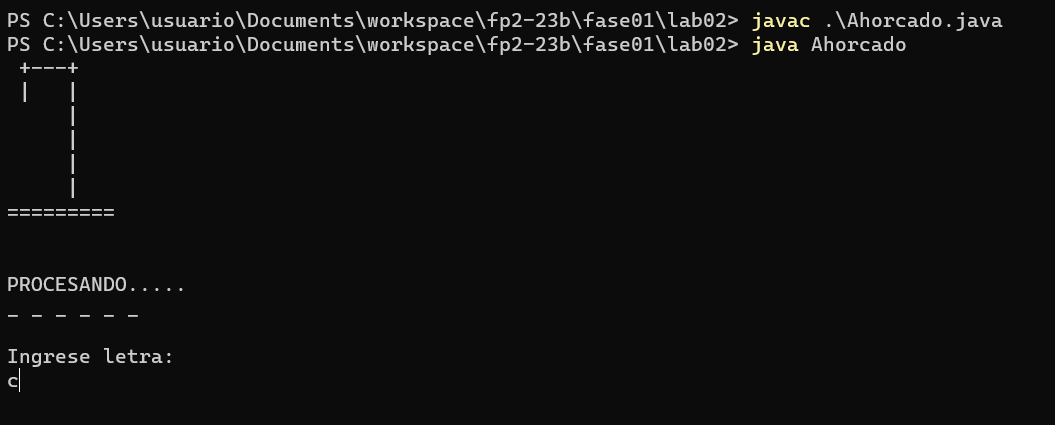
\includegraphics[width=0.8\textwidth,keepaspectratio]{img/captura1.png}
		%\includesvg{img/automata.svg}
		%\label{img:mot2}
		%\caption{Product backlog.}
	\end{figure}
	\begin{itemize}
		\item Al ingresar una letra y acertar hasta terminar la palabra, pasa lo de la siguiente captura.
	\end{itemize}
	\begin{figure}[H]
		\centering
		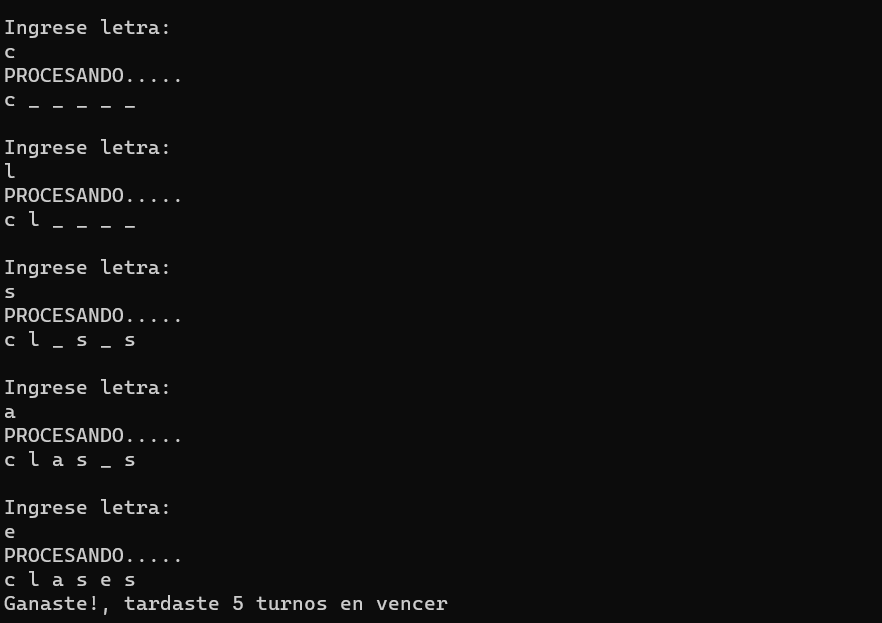
\includegraphics[width=0.8\textwidth,keepaspectratio]{img/captura2.png}
		%\includesvg{img/automata.svg}
		%\label{img:mot2}
		%\caption{Product backlog.}
	\end{figure}
	\begin{itemize}
		\item Y al perder, pasa lo siguiente.
	\end{itemize}
	\begin{figure}[H]
		\centering
		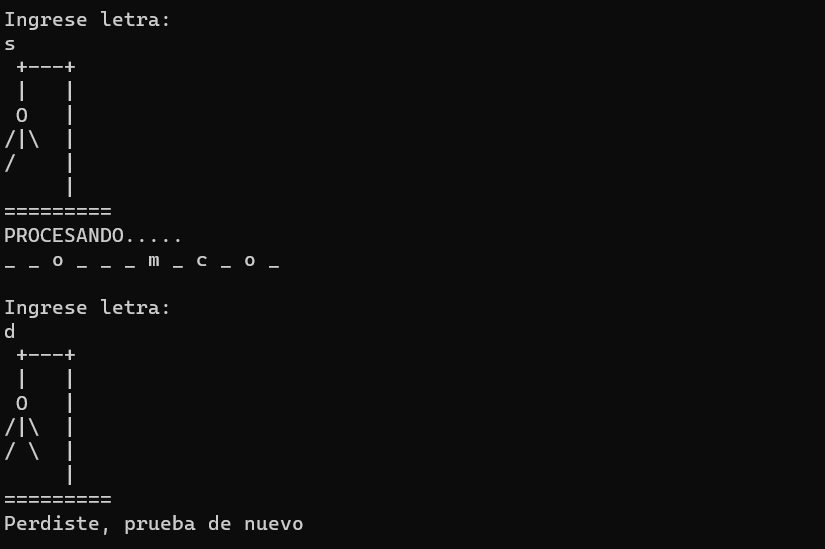
\includegraphics[width=0.8\textwidth,keepaspectratio]{img/captura3.png}
		%\includesvg{img/automata.svg}
		%\label{img:mot2}
		%\caption{Product backlog.}
	\end{figure}
	\section{\textcolor{red}{Rúbricas}}
	
	\subsection{\textcolor{red}{Entregable Informe}}
	\begin{table}[H]
		\caption{Tipo de Informe}
		\setlength{\tabcolsep}{0.5em} % for the horizontal padding
		{\renewcommand{\arraystretch}{1.5}% for the vertical padding
		\begin{tabular}{|p{3cm}|p{12cm}|}
			\hline
			\multicolumn{2}{|c|}{\textbf{\textcolor{red}{Informe}}}  \\
			\hline 
			\textbf{\textcolor{red}{Latex}} & \textcolor{blue}{El informe está en formato PDF desde Latex,  con un formato limpio (buena presentación) y facil de leer.}   \\ 
			\hline 
			
			
		\end{tabular}
	}
	\end{table}
	
	\clearpage
	
	\subsection{\textcolor{red}{Rúbrica para el contenido del Informe y demostración}}
	\begin{itemize}			
		\item El alumno debe marcar o dejar en blanco en celdas de la columna \textbf{Checklist} si cumplio con el ítem correspondiente.
		\item Si un alumno supera la fecha de entrega,  su calificación será sobre la nota mínima aprobada, siempre y cuando cumpla con todos lo items.
		\item El alumno debe autocalificarse en la columna \textbf{Estudiante} de acuerdo a la siguiente tabla:
	
		\begin{table}[ht]
			\caption{Niveles de desempeño}
			\begin{center}
			\begin{tabular}{ccccc}
    			\hline
    			 & \multicolumn{4}{c}{Nivel}\\
    			\cline{1-5}
    			\textbf{Puntos} & Insatisfactorio 25\%& En Proceso 50\% & Satisfactorio 75\% & Sobresaliente 100\%\\
    			\textbf{2.0}&0.5&1.0&1.5&2.0\\
    			\textbf{4.0}&1.0&2.0&3.0&4.0\\
    		\hline
			\end{tabular}
		\end{center}
	\end{table}	
	
	\end{itemize}
	
	\begin{table}[H]
		\caption{Rúbrica para contenido del Informe y demostración}
		\setlength{\tabcolsep}{0.5em} % for the horizontal padding
		{\renewcommand{\arraystretch}{1.5}% for the vertical padding
		%\begin{center}
		\begin{tabular}{|p{2.7cm}|p{7cm}|x{1.3cm}|p{1.2cm}|p{1.5cm}|p{1.1cm}|}
			\hline
    		\multicolumn{2}{|c|}{Contenido y demostración} & Puntos & Checklist & Estudiante & Profesor\\
			\hline
			\textbf{1. GitHub} & Hay enlace URL activo del directorio para el  laboratorio hacia su repositorio GitHub con código fuente terminado y fácil de revisar. &2 &X &2 & \\ 
			\hline
			\textbf{2. Commits} &  Hay capturas de pantalla de los commits más importantes con sus explicaciones detalladas. (El profesor puede preguntar para refrendar calificación). &4 &X &2 & \\ 
			\hline 
			\textbf{3. Código fuente} &  Hay porciones de código fuente importantes con numeración y explicaciones detalladas de sus funciones. &2 &X &2 & \\ 
			\hline 
			\textbf{4. Ejecución} & Se incluyen ejecuciones/pruebas del código fuente  explicadas gradualmente. &2 &X &2 & \\ 
			\hline			
			\textbf{5. Pregunta} & Se responde con completitud a la pregunta formulada en la tarea.  (El profesor puede preguntar para refrendar calificación).  &2 &X &2 & \\ 
			\hline	
			\textbf{6. Fechas} & Las fechas de modificación del código fuente estan dentro de los plazos de fecha de entrega establecidos. &2 &X &2 & \\ 
			\hline 
			\textbf{7. Ortografía} & El documento no muestra errores ortográficos. &2 &X &2 & \\ 
			\hline 
			\textbf{8. Madurez} & El Informe muestra de manera general una evolución de la madurez del código fuente,  explicaciones puntuales pero precisas y un acabado impecable.   (El profesor puede preguntar para refrendar calificación).  &4 &X &4 & \\ 
			\hline
			\multicolumn{2}{|c|}{\textbf{Total}} &20 & &18 & \\ 
			\hline
		\end{tabular}
		%\end{center}
		%\label{tab:multicol}
		}
	\end{table}
	
\clearpage

\section{Referencias}
	
%\clearpage
%\bibliographystyle{apalike}
%\bibliographystyle{IEEEtranN}
%\bibliography{bibliography}
			
\end{document}